\documentclass{article}
\usepackage[utf8]{inputenc}
\usepackage[letterpaper, portrait, margin=1in]{geometry}
\usepackage{multicol}
\usepackage{amsmath}
\usepackage{amssymb}
\usepackage{enumerate}
\setlength\parindent{0pt}
\usepackage{enumerate}
\usepackage{graphicx}
\graphicspath{ {./formula-sheets/images} }
\usepackage{fancyhdr}
\usepackage{tcolorbox}
\usepackage{physics}
\usepackage{enumitem}


\usepackage{calligra}
\DeclareMathAlphabet{\mathcalligra}{T1}{calligra}{m}{n}
\DeclareFontShape{T1}{calligra}{m}{n}{<->s*[2.2]callig15}{}

\newcommand{\sepvec}{\vec{r_\textrm{sep}}}
\newcommand{\sephat}{\hat{r}_{\textrm{sep}}}

\newcommand{\kfrac}{\frac{1}{4\pi\epsilon_0}}

\newcommand{\scripty}[1]{\ensuremath{\mathcalligra{#1}}}


\newcommand{\header}[1]{\begin{large}\noindent #1\end{large}\\\rule{\textwidth}{0.5pt}}
\newcommand{\gap}{\medskip\\}
\newcommand{\centertext}[1]{\begin{center}#1\end{center}}
\newcommand{\bfrac}[2]{\left(\frac{#1}{#2}\right)}
\newcommand{\formula}[3]{\begin{center} \begin{tcolorbox}[title = #2] $$#3$$\end{tcolorbox}\end{center}}
\newcommand{\where}{\hspace{0.5cm} \textrm{where} \hspace{0.5cm}}
\newcommand{\hgap}{\hspace{0.5cm}}
\newcommand{\pfrac}[2]{\frac{\partial #1}{\partial #2}}
\newcommand{\jomega}{{j\omega}}
\newcommand{\domega}{d\omega}

\newcommand{\sheader}[1]{\underline{#1:}}
\newcommand{\smallgap}{\smallskip\\}
\newcommand{\sgap}{\smallskip\\}

\newcommand{\doubleformula}[4]{\begin{center} \begin{tcolorbox}[title = #2] $$#3$$\\$$#4$$\end{tcolorbox}\end{center}}

\newcommand{\tripleformula}[5]{\begin{center} \begin{tcolorbox}[title = #2] $$#3$$\\$$#4$$\\$$#5$$\end{tcolorbox}\end{center}}

\title{PHYS 301 Notes}
\author{reesecritchlow }
\date{September 2022}

\begin{document}

\begin{center}
    \Large PHYS 301 Notes\\
    \normalsize Reese Critchlow
\end{center}

\section*{Midterm 1}

\header{Calculus Review}

\sheader{Spherical Coordinates}
\smallskip\\
Sometimes, spherical coordinates are easier to work with than cartesian coordinates.
When using spherical coordinates, there are some key things to note:
\begin{enumerate}
    \item \sheader{The coordinates themselves:} 
    \smallgap
    $\phi$: Equatorial Azimuth $[0, 2\pi]$ (from the ``$x$'' axis)\\
    $\theta$: Axial Azimuth $[0, \pi]$ (from the ``$z$'' axis)\\
    $r$: Radial Distance
    \item \underline{The infinitesimal displacement is different:}
    \smallgap
    $d\vec{l} = dr \, \hat{r} + r d\theta \, \hat{\theta} + r \sin \theta d\phi \, \hat{\phi}$
    \item \underline{The volume element is different:}
    \smallgap
    $d\tau = r^2 \sin \theta \, dr \, d\theta \, d\phi$
\end{enumerate}

\sheader{Cylindrical Coordinates:} See textbook, this would be too redundant.
\gap
\sheader{Rules for Irrotational Fields/Conservative Fields}
\begin{enumerate}
    \item $\vec{\nabla} \times \vec{F} = \vec{0}$ everywhere.
    \item $\int_a^b\vec{F}\cdot d\vec{l}$ is independent of path, for any given end points.
    \item $\oint \vec{F}\cdot d\vec{l} = 0$ for any closed loop.
    \item $\vec{F}$ is the gradient of some scalar function: $\vec{F} = -\nabla V$.
\end{enumerate}
It is important to note that since $\vec{E} = -\nabla V$, then all electrostatic fields 
are irrotational.
\sgap
\sheader{Rules for Divergence-less fields.}
\begin{enumerate}
    \item $\vec{\nabla} \cdot \vec{F} = 0$ everywhere.
    \item $\int \vec{F} \cdot d\vec{a}$ is independent of surface, for any given boundary line.
    \item $\oint \vec{F} \cdot d\vec{a} = 0$ for any closed surface.
    \item $\vec{F}$ is the curl of some vector function.
\end{enumerate}
\sheader{Taylor Expansions} Often, it is difficult to obtain limits for when one quantity
gets significantly larger than another in equations describing fields or potentials.
Thus, the \underline{Taylor Expansion} is helpful for this. Take for example a quantity $a$
and a quantity $b$. For $b >> a$, it is useful to try to bring the equation into a form
such that $\left(\frac{a}{b}\right)^n, n \in \mathbb{N}$. Since $b >> a$, then we can say that $\frac{a}{b} \approx 0$
Thus, a Taylor series centered around $x = 0$ is obtained, which can be evaluated with
the expression:
\[
    f(x) \approx f(0) + f'(0) \cdot x  + f''(0) \cdot \frac{x^2}{2} + \cdots + \frac{f^{(n)}x^n}{n!}   
\]
Generally, it is best practice to evaluate the Taylor series up until the degree of the
largest polynomial in the original function.

\pagebreak
\header{Electric Fields}

It is important to recognize the notation in the Griffith's textbook, which is used
primarily for this course when working with Fields and directions:
\sgap
$\vec{r}$: distance from the origin to a ``field point''.\\
$\vec{r'}$: distance from the origin to the charge\\
$\sepvec$ : distance from the charge to the ``field point''\\
Thus, it is given that $\sepvec = \vec{r} - \vec{r'}$.
\gap
Now, while working with Coulomb's law, we can define the electric field due to a point charge to be:
\[
    \vec{E} = \frac{1}{4\pi \epsilon_0} \frac{q}{||\sepvec||^2}\sepvec    
\]
\sheader{Types of Field Integrations} There exist three main types of field integrations:
\begin{multicols}{3}
    \centertext{\underline{Line Charge}}
    \[
        \vec{E}(\vec{r}) = \frac{1}{4 \pi \epsilon_0}\int{\frac{\lambda(\vec{r'})}{||\sepvec||^2}\sephat \, dl'}    
    \]
    \vfill\null\columnbreak
    \centertext{\underline{Surface Charge}}
    \[
        \vec{E}(\vec{r}) = \frac{1}{4\pi\epsilon_0}\int{\frac{\sigma(\vec{r'})}{||\sepvec||^2}\sephat \, da'}    
    \]
    \vfill\null\columnbreak
    \centertext{\underline{Volume Charge}}
    \[
        \vec{E}(\vec{r}) = \frac{1}{4\pi\epsilon_0}\int{\frac{\rho(\vec{r'})}{||\sepvec||^2}\sephat \, d\tau'}    
    \]
    \vfill\null
\end{multicols}
\sheader{Gauss's Law} Gauss's law is as follows:
\begin{align*}
    \oint{\vec{E} \cdot d\vec{a}} = \frac{Q_\textrm{encl}}{\epsilon_0} && \vec{\nabla} \cdot \vec{E} = \frac{\rho}{\epsilon_0}
\end{align*}
By knowing the geometry and symmetry of a situation however, Gauss's law can require
no integration whatsoever. This is when we know that field is the same for every point
on a surface. 
\gap
\header{Electric Potential}
The potential of a point in a field relative to another is defined as:
\[
    V(\vec{r}) \equiv - \int_{\mathcal{O}}^r \vec{E} \cdot d\vec{l}    
\]
Which is often referred to as the potential difference between two points:
\[
    V(\vec{b}) - V(\vec{a}) = - \int_{\vec{a}}^{\vec{b}}{\vec{E} \cdot d\vec{l}}
\]
It is also to be noted the relation between field and potential:
\[
    \vec{E} = - \nabla V    
\]
\sheader{Remark} it is important to note that unlike electric field, electric potential
is a \underline{scalar}. It has no direction, and should be handled accordingly.
\gap
Potential can also be obtained for a volume charge:
\[
    V(\vec{r}) = \kfrac \int{\frac{\rho(\vec{r'})}{||\sepvec||}d\tau'}
\]
Similar formulae can be extrapolated for line and surface charge distributions, analogous
to those for electric fields.
\gap
However, the formula for point charges is important to note:
\[
    V(\vec{r}) = \kfrac \sum_{i = 0}^n\frac{q_i}{||\sepvec||}
\]
\pagebreak
\gap
\header{Work and Energy in Electrostatics}
To calculate the work that it takes to get from one point to another in a field,
we can use a \underline{work integral}. We can also employ the potential difference.
\[
    W = \int_{\textbf{a}}^{\textbf{b}} \vec{F} \cdot d\vec{l} = -Q\int_{\textbf{a}}^{\textbf{b}}{\vec{E} \cdot d\vec{l}} = Q[V(\vec{b}) - Q(\vec{a})]
\]
It is important to note that for the second form of this integral uses \textbf{negative} $Q$,
not positive. This is because the integral by default describes the amount of work that
the \underline{field does}, not the work that \underline{is required}. One can use 
a positive value of $Q$ if trying to find out how much work the field does.
\gap
It is also to be noted that the potential of a system is the work that is required
to create the system \underline{per unit charge}.
\gap
\sheader{Work and Point Charges} We can also describe the amount of work that it takes
to assemble a collection of point charges:
\[
    W = \frac{1}{2}\sum_{i = 1}^n{q_i V(\vec{r_i})}    
\]
\sheader{Work of a Continuous Charge Distribution} To describe the amount of energy
that a charge distribution has, or the amount of energy required to create it in 
empty space, the following formula can be used:
\[
    W = \frac{\epsilon_0}{2}\int\limits_{\textrm{all space}}E^2 d\tau    
\]

\header{Boundary Conditions}
One of the important equations in the relationships between $\rho$, $V$, and $E$ is 
$\nabla^2 V = - \frac{\rho}{\epsilon_0}$. However, this equation often leaves one 
with a number of undetermined coefficients from the integration. Thus, it is important
to investigate the boundary conditions of fields and potentials.
\gap
From this, a set of important boundary conditions emerges for a boundary at $a$.
\begin{itemize}
    \item \sheader{Continuity of Potential} Since $\nabla V = -\vec{E}$, it is known 
    that potential should be continuous along all space. Thus,
    \[
        V_\textrm{above}(a) = V_\textrm{below}(a)
    \]
    \item \sheader{Preservation of Field} For any field interacting with a surface charge,
    by Gauss's law, it is known that the difference between the field above and the field
    below is simply the surface charge density over the permittivity of free space:
    \[
        \vec{E}_\textrm{above} - \vec{E}_\textrm{below} = \frac{\sigma}{\epsilon_0}\hat{n}    
    \]
    Where $\hat{n}$ is the normal vector of the boundary surface. The presence of the
    normal vector is important, because it requires the boundary surface to have 
    symmetry with the field above and the field below.
    \item \sheader{Bounding of Potential (not general)} Since it is known that potential should generally 
    be bounded over all space (except in some cases), it is appropriate to say that
    \[
        V(0) \textrm{ is bounded.}    
    \]
    This is generally more true for configurations with spherical symmetry.
    \item \sheader{Zero Potential at Infinity (not general)} For many spherically-symmetric
    examples, it is known that the potential at infinity is zero. Thus, it can be said that:
    \[
        V(\infty) = 0.    
    \]
\end{itemize}
\pagebreak

\header{Uniqueness of Solutions}
Given the relationship $\nabla^2 V = -\frac{\rho}{\epsilon_0}$, there exists the case
that $\rho =0$, for which a distinct set of attributes arise:
\begin{enumerate}
    \item $V$ has no local maxima nor minima inside. The maxima and minima are located
    on the surrounding boundaries.
    \item $V$ is smooth and continuous, everywhere.
    \item $V(\vec{r})$ is the average of $V$ over surface of any surrounding sphere:
    $V(\vec{r}) = \frac{1}{4\pi R^2}\oint VdA$.
    \item $V$ is unique, as the solution of the Laplace equation is uniquely determined
    if $V$ is specified on the boundary surface around the volume.
\end{enumerate}

\sheader{Earnshaw's Theorem} As a sidenote, is important to note \underline{Earnshaw's Theorem},
which states that: 
\centertext{A charged particle cannot be held in a stable equilibrium by electrostatic forces alone.}
This can be analyzed using divergence amongst other methods of analysis.
\gap
\header{Conductors}
At a base level, conductors are materials in which electrons are free to move inside 
of the material. Because of this, [ideal] conductors are able to rearrange their
charges, allowing them to have special properties:
\begin{enumerate}
    \item \underline{$\vec{E} = 0$ inside a conductor}. In short, charges move to oppose any external $\vec{E}$ fields.
    This can also be interpreted under the principle that if there was any field inside
    a conductor, the free electrons would be moving, and hence not \textit{electrostatic}.
    \item \underline{Any net charges reside on the surface of a conductor.}
    \item \underline{$\rho = 0$ inside a conductor}. Since there is no field inside a conductor,
    Gauss's law requires that there is no enclosed charge, thus, there is no charge density.
    One may make the argument for the surface charges, however, since they are equal in magnitude,
    they cancel.
    \item \underline{A conductor is an equipotential}. Since there is no field inside
    a conductor, given the relationship $\nabla V = -\vec{E}$, the potential $V$ must
    be a constant.
    \item \underline{$\vec{E}$ is normal to the surface of a conductor.} This is because
    any non-normal direction of field would result in fields inside the conductor. (Unsure of this)
\end{enumerate} 

\header{Capacitance}

As a purely geometrical property, we can define \textbf{capacitance} as the ratio of
charge to voltage. Thus, it is defined as:
\[
    C \equiv \frac{Q}{V}.    
\]
As a practical device, \underline{capacitors} are capable of storing energy. Thus, it
is important to define the amount of energy that a capacitor can store for a given 
charge $Q$ and capacitance $C$:
\begin{align*}
    W = \int_0^Q{\bfrac{q}{C}dq} = \frac{1}{2}\frac{Q^2}{C} = \frac{1}{2} CV^2
\end{align*}

\pagebreak

\section*{Midterm 2}

\header{Multipole Expansion}

It can be said that every charge distribution has characteristics of 
various multipoles at large distances. Thus, we can utilize the \underline{multipole expansion}
to determine voltages at large distances.

\[
    V(r) = \frac{1}{4\pi \epsilon_0}\sum_{n = 0}^\infty \frac{1}{r^{n + 1}} \int_{V} ||\vec{r'}|| P_n(\cos \alpha)\rho(\vec{r'})d\tau'   
\]

Where $\alpha$ is the angle between the reference and separation vectors.
\gap
However, it is to be noted that this formula is often very difficult to use. Thus,
we can isolate the first two terms, which are generally of the most use to us.
\[
    V \approx \frac{1}{4\pi\epsilon_0}\frac{Q}{r} + \frac{1}{4\pi \epsilon_0} \frac{\vec{p} \cdot \hat{r}}{r^2} + \cdots
\]
The first term in the sequence is the \underline{monopole} term and the second term in 
the sequence is the \underline{dipole} term. Thus, we also define $Q$ as the total charge
of the charge distribution under analysis and $\vec{p}$ as the \underline{dipole moment} 
of the distribution. The dipole moment is described by:
\[
    \vec{p} \equiv \int_V \vec{r'}\rho(\vec{r'})d\tau'   
\]

We can also describe dipole moment for a collection of point charges as well:
\[
    \vec{p} = \sum_{i = 1}^n q_i \vec{r'}_i    
\]

Lastly, we can also define the dipole moment for a dipole that is not centered at the origin.
\[
    \vec{p'} = \vec{p} - Q\vec{a}  
\]
for a shift of $\vec{a}$ from the origin.
\gap
\header{Polarization and Dielectrics}

Polariztion occurs when an electric field passes through a \underline{dielectric}, which
is an insulator. Because the charges in a dielectric are not free to roam like in a 
conductor, the charges tend to ``strech'' and ``rotate'', which produce different behaviours.
\gap
In atoms with no permanent dipole, the electrons and nucleus will rearrange such that a 
dipole is \underline{induced} into the atom. In molecules with permanent dipoles, however,
they experience a \underline{torque}, which can be described by 
\[
    \vec{N} = \vec{p} \times \vec{E}    
\]
That being said, there could also be a nonuniform field, and thus a nonuniform force distribution,
resulting in a net force, described by:
\[
    \vec{F} = (\vec{p} \cdot \nabla)\vec{E}.   
\]
We can also describe the energy of an ideal dipole in an electric field:
\[
    U = -\vec{p} \cdot \vec{E}.    
\]

\pagebreak

\header{Bound and Free Charges}

As a result of polarization, we can describe the phenomena known as \underline{bound charges}
and \underline{free charges}. 
\gap
\underline{Bound Charges} are charges that are produced when the ``stretching'' effect
of an electric field results in charges moving to the outer surfaces of an object. We 
can define such surface charges as:
\[
    \sigma_\textrm{bound} = \vec{P} \cdot \hat{n}.    
\]
Additionally, we can also define the charge density of the bound charges:
\[
    \rho_\textrm{bound} \equiv -\nabla \cdot \vec{P}    
\]
It is important to note that such bound charges create electric fields within the dielectric
itself. Thus, the total electric field inside of a dielectric is described by:
\[
    \vec{E}_d = \vec{E}_\textrm{outside} + \vec{E}_\textrm{inside}    
\]
\underline{Free Charge} is the charge on an object that is ``externally applied''. It 
is not generated by polarization.
\gap
\header{Electric Displacement}

Electric displacement is the vector field representing how bound charges separate within 
a material. It is defined as:
\[
    \vec{D} \equiv \epsilon_0 \vec{E} + \vec{P}.    
\]
Electric displacement can also be described using Gauss's law, which follows the form of:
\begin{align*}
    \nabla \cdot \vec{D} = \rho_f && \oint\vec{D} \cdot d\vec{A} = Q_{f_\textrm{encl}}
\end{align*}
These expressions are convenient because free charges are the ones that ``we control''.
\gap
\sheader{Remark} There is an important condition that comes into play when using Gauss's
law with displacement fields. This has to do with the fact that \underline{the curl of a displacement field is not always zero}.
This is because the way in which the field is generated is not in the same irrorational
sense as electric fields. Thus, since Gauss's law is application of Divergence Theorem, 
Gauss's law for electric displacement \underline{does not hold} when $\nabla \times \vec{D} \neq 0$.
\gap
\sheader{Avoiding Error} Per Griffiths, if the problem has spherical, cyclindrical, or planar
symmetry, $\vec{D}$ can be obtained by by the usual Gauss's law methods. Additionally,
due to the definition, instead of checking if $\nabla \times \vec{D} \neq 0$, we can also check
that:
\[
    \nabla \times \vec{P} \neq 0.
\]
\sheader{Boundary Conditions} We can also define a new boundary condition for electric displacement
questions:
\[
    D_\textrm{above}^\perp - D_\textrm{below}^\perp = \sigma_\textrm{free}.
\]

\header{Linear Dielectrics}

It is known that for some materials, the polarization can be described as proportional to
the electric field that the material is experiencing. The relationship, which is described
by:
\[
    \vec{P} = \epsilon_0 \chi_e \vec{E}
\]
introduces the constant $\chi_e$, which is the \underline{electric susceptibility} of the
material. Materials that obey this relationship are called \underline{linear dielectrics}.
\gap
This relationship can be also rewritten as:
\[
    \vec{D} = \epsilon \vec{E}
\]
where, 
\[
    \epsilon = \epsilon_0 (1 + \chi_e) = \epsilon_0 \epsilon_r.    
\]
We also define the quantity $\epsilon_r$, as the \underline{relative permittivity} or 
\underline{dielectric constant} of the material.

\pagebreak

\header{Laplace Equations in Cartesian Coordinates}

Laplace equations are helpful to solve problems where planar boundary conditions exist.
They exploit the fact that the solution follows a separable form. Since we've seen these 
before [reference MATH 257 notes], we only require some basic review.
\begin{enumerate}
    \item Solutions will have a hyperbolic trig function or a sinusoidal trig function.
    the difference between the two depends on boundary conditions.
    \begin{enumerate}
        \item Boundaries that start and end at the same value generally will be 
        sinusoidal function solutions.
        \item Boundaries that start and end at different values generally will beam
        hyperbolic trigonometric function solutions.
        \begin{itemize}
            \item $\sinh(0) = 0$
            \item $\cosh(0) = 1$
        \end{itemize}
    \end{enumerate}
    \item To find coefficients in a Fourier series, we use the length of that dimension 
    to integrate over. 
\end{enumerate}

\header{Laplace Equations in Spherical Coordinates}

Laplace equations in spherical coordinates are helpful for solving problems with complicated
external factors and spherical symmetry. They yield solutions that take the form of:
\[
    f(r, \theta) = R(r) \Theta(\theta).
\]
Working through the steps of the laplace equation, we obtain that this form looks like:
\[
    f(r, \theta) = \sum_{l = 0}^\infty{\left(A_l r^l + \frac{B_l}{r^{l + 1}}\right)P_l(\cos \theta)}.    
\]
Where $P_l(\cos \theta)$ are associated \underline{Legendre polynomials}, which have the form:
\begin{align*}
    P_0(\cos \theta) &= 1\\
    P_1(\cos \theta) &= \cos\theta \\
    P_2(\cos \theta) &= \frac{3}{2} \cos^2 \theta - \frac{1}{2}\\
    P_3(\cos \theta) &= \frac{5}{2} \cos^3 \theta - \frac{3}{2} \cos \theta
\end{align*}

\sheader{Boundary Conditions} There exist a particular set of boundary conditions that are 
often helpful when solving problems involving laplace equations in spherical coordinates:
\begin{enumerate}
    \item \sheader{Bounding of Potential at Zero} $V(r = 0) = $ finite
    \item \sheader{Bounding of Potential at Infinity} $V(r \to \infty) = V_0$
    \item \sheader{Continuity of Field} (Linear, Internal Dielectrics) 
    $\eval{\epsilon_r \frac{\partial V_\textrm{in}}{\partial r}}_{r = R} = \eval{\frac{\partial V_\textrm{out}}{\partial r}}_{r = R}$\\
    or $\eval{\frac{\partial V_\textrm{above}}{\partial r}}_{r = R} - \eval{\frac{\partial V_\textrm{below}}{\partial r}}_{r = R} = \frac{\sigma}{\epsilon_0}$
    \item \sheader{Continuity of Potential} $V_\textrm{in} = V_\textrm{out}$
\end{enumerate}

\sheader{Solving Spherical Laplacian Problems}
\begin{enumerate}
    \item Employ bounding boundary conditions [(1) and (2)].
    \item Match terms with continuity of potential.
    \item Match terms with continuity of electric field.
\end{enumerate}

\pagebreak

\header{Method of Images}
The \underline{method of images} is used to solve problems involving charge distributions
and large, grounded sheets. Generally, a ``mirror charge'' is required in such cases, 
although the following formula may be of use:
\[
    V(r = a, \theta) = \frac{1}{4\pi \epsilon_0} \left(\frac{q_1}{||\vec{r_1}_\textrm{sep}||} + \frac{q_2}{||\vec{r_2}_\textrm{sep}||}\right) = 0
\]
Solving the equation of
\[
    -\frac{q_1}{q_2} = \frac{||\vec{r_1}_\textrm{sep}||}{||\vec{r_2}_\textrm{sep}||}
\]
will allow one to determine the location and charge magnitude of corresponding image charges.
\gap
It is also important to note that the following formula may be useful in finding the 
surface charge of the grounded plane:
\[
    \sigma = - \epsilon_0 \frac{\partial V}{\partial n}
\]
where $n$ is the normal direction of the surface which is being integrated over.

\section*{Final Exam}

\header{Magnetic Fields}
Moving charges generate not only electric fields but also magnetic fields.
This magnetic field produces a magnetic force on an object, which can be
described by the \textbf{Lorentz force law}:
\begin{align*}
    \vec{F}_\textrm{mag} = Q(\vec{v} \times \vec{B})
\end{align*}
It is important to note that the Lorentz force law implies that 
\textbf{magnetic forces do no work}.
\gap
\header{Currents}
The \textbf{current} in an object is the \underline{charge per unit time}
passing through a given point. It is measured in amperes, which are coulombs-per-second.
We can also define other dimensions of current:
\gap
\sheader{Surface Current Density} Surface current density, described by $\vec{K}$
describes the current in an ``infinitesimal ribbon'' across the surface
of an object. Hence, for some ``infinitesimal ribbon'' with width $dl_\perp$,
with current inside of it $d\vec{I}$, then we can define $\vec{K}$ as:
\begin{align*}
    \vec{K} \equiv \frac{d\vec{I}}{dl_\perp}.
\end{align*}
In other words, $\vec{K}$ is the \underline{current per unit width}. We 
can also define it in terms of surface current density:
\begin{align*}
    \vec{K} = \sigma \vec{v}
\end{align*}
\sheader{Volume Current Density} Volume current density, described by $\vec{J}$
can be thought of as the current flowing through some ``infinitesimal tube'' 
of area $da_\perp$. Hence, the current in this tube can be thought of as 
$d\vec{I}$, and thus $\vec{J}$ is defined as:
\begin{align*}
    J \equiv \frac{d\vec{I}}{da_\perp}
\end{align*}
Hence, the same analgies can be drawn, $\vec{J}$ is the \underline{current per unit area}
and we can also describe it as:
\begin{align*}
    \vec{J} = \rho\vec{v}.
\end{align*}
From these definitions, we can find the magnetic force for all of these current
configurations:
\begin{align*}
    \vec{F}_\textrm{mag} = \int I(d\vec{I} \times \vec{B}) &&
    \vec{F}_\textrm{mag} = \int (\vec{K} \times \vec{B})da &&
    \vec{F}_\textrm{mag} = \int (\vec{J} \times \vec{B}) d\tau.
\end{align*}

\pagebreak
\header{The Biot-Savart Law}
The Biot-Savart Law describes the field that results from a steady charge.
As axioms of this, we require that $\frac{\partial \vec{J}}{\partial t} = \vec{0}$
and as a consequence, $\vec{\nabla} \cdot \vec{J} = 0$.
\gap
Hence, to calculate magnetic fields, we use the \underline{Biot-Savart Law}:
\begin{align*}
    \vec{B}(\vec{r}) = \frac{\mu_0}{4\pi} \int \frac{\vec{I} \times \hat{r}_\textrm{sep}}{||\sepvec||^2} dl' = 
    \frac{\mu_0}{4\pi}I \int \frac{d\vec{I}'\times \hat{r}_\textrm{sep}}{||\sepvec||^2}
\end{align*}

The integration is along the path of the current and in the direction of the flow.
$d\vec{I}'$ is an element of length along the wire. 
\gap
Hence, we define the units of measurement for magnetic field to be in Teslas,
which are newtons per ampere-meter:
\begin{align*}
    1 \,\,\textrm{T} = 1 \, \,\textrm{N}(\textrm{A} \cdot \textrm{m})
\end{align*} 
\header{Ampere's Law}
The derivation of Ampere's law has some interesting implications. The first,
is that the divergence of $\vec{B}$ is zero:
\begin{align*}
    \vec{\nabla} \cdot \vec{B} = 0
\end{align*}
\begin{center}
    \underline{\textbf{Since a magnetic monopole does not exist, all magnetic fields are divergence-less.}}
\end{center}
The next is the curl of $\vec{B}$:
\begin{align*}
    \vec{\nabla} \times \vec{B} = \mu_0\vec{J}.
\end{align*}
\begin{center}
    \underline{\textbf{Since magnetic fields always form loops, then those loops, and their subsequent curl}}\\
    \underline{\textbf{ must come from currents and changing electric fields.}}
\end{center}
Finally, from this we can also find the integral form of the curl:
\begin{align*}
    \oint \vec{B} \cdot d\vec{l} = \mu_0 I_\textrm{encl}.
\end{align*}

Ampere's law generally is used for a small subset of problems:
\begin{enumerate}
    \item Infinite straight lines
    \item Infinite planes
    \item Infinite solenoids
    \item Toroids
\end{enumerate}

\header{Magnetic Vector Potential}

Similar to how the gradient of the voltage produces the electric field in 
electrostatics, there exists a vector potential, $\vec{A}$ in magnetostatics.
\begin{align*}
    \vec{B} = \vec{\nabla} \times \vec{A}.
\end{align*}
This also implies that:
\begin{align*}
    \vec{\nabla} \cdot \vec{A} = 0
\end{align*}

Through some math, we can find a Poisson's equation in magnetostatics:
\begin{align*}
    \nabla^2 \vec{A} = -\mu_9 \vec{J}.
\end{align*}
Which, with the assumption that $\vec{J}$ goes to zero at infinity, we obtain that:
\begin{align*}
    \vec{A}(\vec{r}) = \frac{\mu_0}{4\pi} \int \frac{\vec{J}(\vec{r'})}{||\sepvec||}d\tau'.
\end{align*}

\pagebreak
We can also expand this to line and surface currents:
\begin{align*}
    \vec{A} = \frac{\mu_0}{4\pi} \int \frac{\vec{I}}{||\sepvec||}dl' = \frac{\mu_0 I}{4\pi} \int \frac{1}{||\sepvec||}d \vec{l}' && \vec{A} = \frac{\mu_0}{4\pi}\int \frac{\vec{K}}{||\sepvec||}da'
\end{align*}
Typically, the vector potential $\vec{A}$ mimics the direction of the current. 
\gap
\header{The Triangle of Magnetostatics}
\begin{center}
    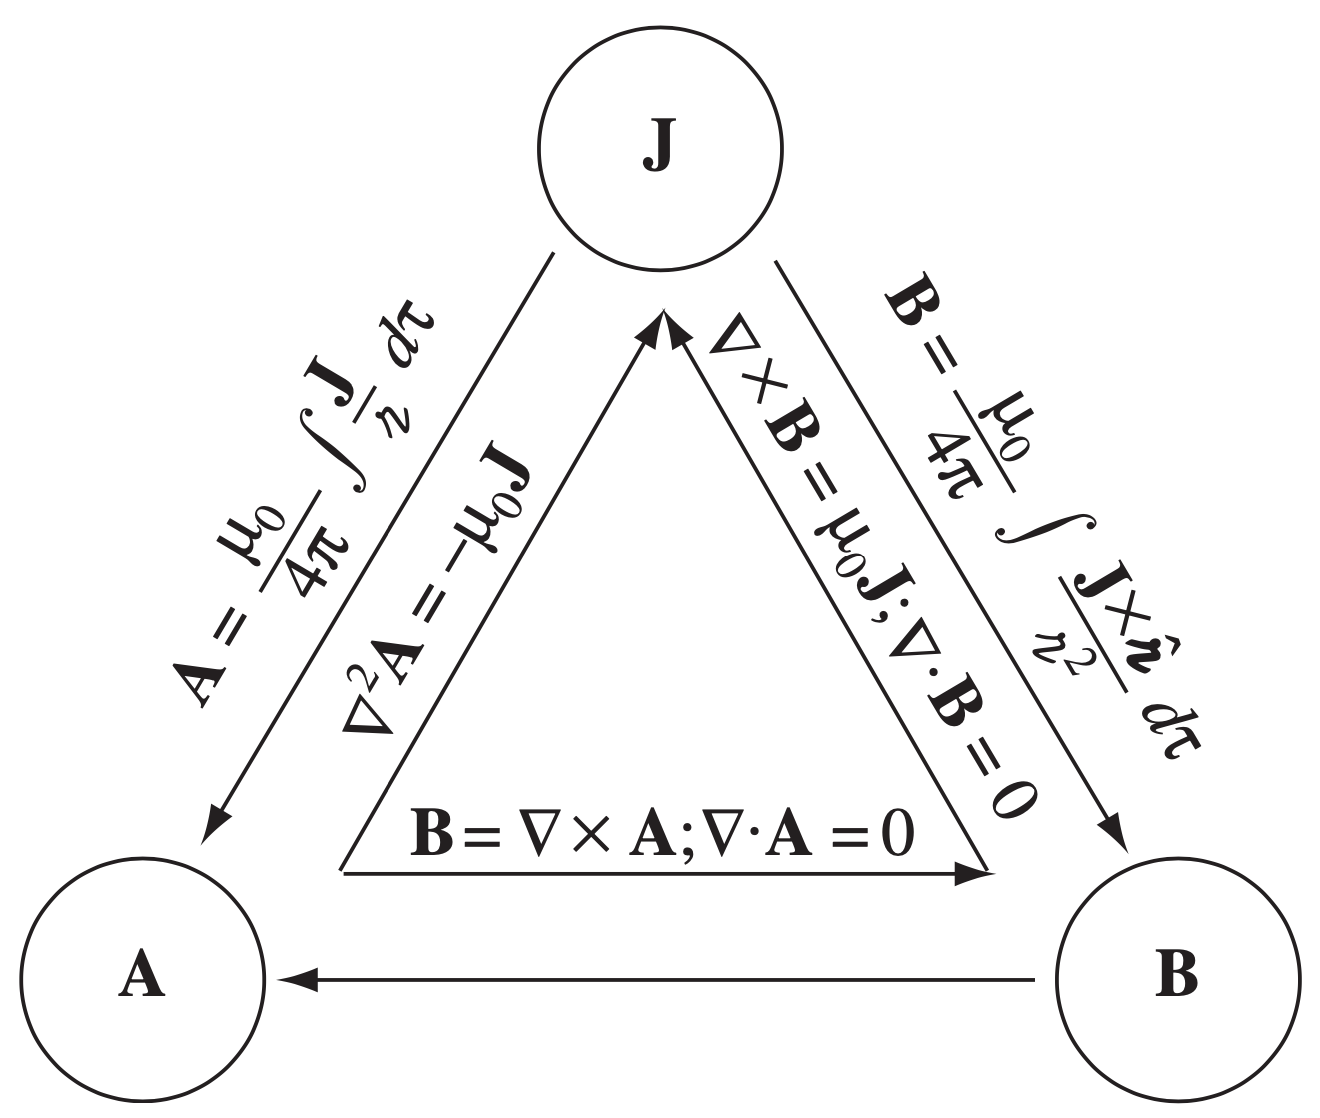
\includegraphics[scale=0.35]{magnetic-triangle.png}
\end{center}
\header{Boundary Conditions}
There also exist a set of boundary conditions for magnetostatics:
\begin{enumerate}[label=(\alph*)]
    \item $B_\textrm{above}^\perp = B_\textrm{below}^\perp$
    \item $B_\textrm{above}^\parallel - B_\textrm{below}^\parallel = \mu_0 K$
    \item $\vec{B}_\textrm{above} - \vec{B}_\textrm{below} = \mu_0 (\vec{K} \times \hat{n})$
    \item $\vec{A}_\textrm{above} = \vec{A}_\textrm{below}$
    \item $\frac{\partial \vec{A}_\textrm{above}}{\partial n} - \frac{\partial \vec{A}_\textrm{below}}{\partial n} = - \mu_0 \vec{K}$
\end{enumerate}

\header{Multipole Expansion of the Vector Potential}
There also exists a multipole expansion for the vector potential. The principle with the 
cosine law is the same as in electrostatics.
\sgap
First, we define the \underline{magnetic dipole moment}, $\vec{m}$ to be:
\begin{align*}
    \vec{m} \equiv I \int d\vec{a} = I \vec{a}
\end{align*}
Where $\vec{a}$ is the ``vector area'' of the loop, where the area of the loop is it's 
magnitude, and the direction is the normal direction of the loop, based on current
and the right hand rule.
\sgap
Since there exists no monopole in magnetostatics, the choice of origin is irrelevant in 
magnetostatics. 
\sgap
With this information, we can find the potential of a magnetic dipole:
\begin{align*}
    \vec{A}_\textrm{dip}(\vec{r}) = \frac{\mu_0}{4\pi} \frac{\vec{m} \times \hat{r}}{r^2}.
\end{align*}





\end{document}